% ============================================================================
% Section V: Experiments
% ============================================================================
% Centralized statistics used by Section/experiments.tex.
% All standard deviations are sample standard deviations (ddof=1).

\def\ChenNSGAMean{0.3222}
\def\ChenNSGAStd{0.0237}
\def\ChenParEGOMean{0.3853}
\def\ChenParEGOStd{0.0094}
\def\ChenLLMBOMean{0.3835}
\def\ChenLLMBOStd{0.0079}
\def\ChenLLMBODelta{-0.0018}
\def\ChenLLMBORelative{-0.46\%}
\def\ChenLLMBOWins{2/5}
\def\ChenLLMBOStdReduction{15.7\%}

\def\EckerParEGOMean{1.5866}
\def\EckerParEGOStd{0.0130}
\def\EckerLLMBOMean{1.8684}
\def\EckerLLMBOStd{0.0027}
\def\EckerLLMBODelta{0.2819}
\def\EckerLLMBORelative{17.77\%}
\def\EckerLLMBOWins{5/5}

\def\AblationBaselineMean{0.3836}
\def\AblationBaselineStd{0.0113}
\def\AblationWarmMean{0.3902}
\def\AblationWarmStd{0.0087}
\def\AblationWarmDelta{0.0066}
\def\AblationRegionMean{0.3862}
\def\AblationRegionStd{0.0125}
\def\AblationRegionDelta{0.0026}
\def\AblationFullMean{0.3900}
\def\AblationFullStd{0.0067}
\def\AblationFullDelta{0.0064}


\section{Experiments}
\label{sec:experiments}

\subsection{Experimental Protocol}

All results in this section are obtained in simulation; no new cell tests are
reported. The simulator is the PyBaMM SPMe implementation described in
Section~\ref{sec:model}, with lumped thermal dynamics and the empirical aging
term used by the optimizer. We study the 5-A LG INR21700-M50 parameterization
(Chen2020)~\cite{ref13} and the 0.156-Ah Kokam SLPB~75106100
parameterization (Ecker2015)~\cite{ref14}. In both cases, the optimizer
minimizes charging time, peak temperature rise, and capacity fade for the
five-variable multistage protocol defined in Section~\ref{sec:problem}.

Each BO run contains six initialization evaluations followed by 50
iterations, for a total of 56 simulator calls. Results are paired over seeds
8409--8413. ParEGO uses the archived MATLAB-reference scalarization and
acquisition settings. The Chen2020 study also includes NSGA-II; its archived
60-evaluation run is replayed only through evaluation 56 in the quality
comparison. LLMBO-MO uses three screened LLM proposals and three random
initial points. The Chen2020 comparison uses DeepSeek-V3, whereas the
Ecker2015 transfer run uses DeepSeek-V3-Thinking; both use temperature zero
and one completion. Thus, the cross-cell experiment evaluates transfer of
the optimization workflow, not invariance to the LLM backend.

\subsubsection{Hypervolume reporting}
The archive key \texttt{canonical\_hv} is reported here as
\emph{benchmark-scaled hypervolume} (sHV). For objective vector
$\mathbf f=[t_c,\Delta T_p,Q_s]^\top$, define
\begin{equation}
\tilde{\mathbf f}
=
[\log_{10}t_c,\ \Delta T_p,\ \log_{10}Q_s]^\top .
\end{equation}
For benchmark $b$, sHV is
\begin{equation}
\mathrm{sHV}_b(\mathcal P)
=
\frac{\mathrm{HV}(\tilde{\mathcal P};\tilde{\mathbf r}_b)}
{\prod_{i=1}^{3}(\tilde r_{b,i}-\tilde z_{b,i})},
\label{eq:scaled_hv}
\end{equation}
where $\mathbf z_b$ and $\mathbf r_b$ are fixed nominal ideal and reference
points. Chen2020 uses $[1800,0,0.3]$ and $[7200,40,5]$; Ecker2015 uses
$[2500,0,0.2]$ and $[7000,35,4.5]$. No clipping is applied. Consequently,
sHV is dimensionless but is not constrained to $[0,1]$ when an observation
improves on the nominal ideal point. Absolute sHV values are therefore
compared only within a benchmark. Curves show the mean and sample standard
deviation over five seeds.

\subsection{Fixed-Budget Benchmark Results}

Table~\ref{tab:benchmark_results} and Fig.~\ref{fig:benchmark_hv} summarize
the matched five-seed runs. The Chen2020 result does not show a mean advantage
over ParEGO: LLMBO-MO finishes at \ChenLLMBOMean, compared with
\ChenParEGOMean\ for ParEGO, a difference of \ChenLLMBORelative. Its
seed-to-seed standard deviation is \ChenLLMBOStd\ rather than
\ChenParEGOStd, a reduction of \ChenLLMBOStdReduction. LLMBO-MO wins two of
the five paired seeds. We therefore treat the Chen2020 result as comparable
final quality with lower variation, not as an improvement in mean sHV.

\begin{table}[!t]
\caption{Fixed-Budget Benchmark Results over Five Seeds}
\label{tab:benchmark_results}
\centering
\footnotesize
\setlength{\tabcolsep}{3.2pt}
\begin{tabular}{@{}llccc@{}}
\toprule
Cell model & Method & Evals. & Final sHV & Wins \\
\midrule
\multirow{3}{*}{Chen2020}
& NSGA-II & 56 & \ChenNSGAMean\,$\pm$\,\ChenNSGAStd & -- \\
& ParEGO & 56 & \textbf{\ChenParEGOMean}\,$\pm$\,\ChenParEGOStd & -- \\
& LLMBO-MO & 56 & \ChenLLMBOMean\,$\pm$\,\textbf{\ChenLLMBOStd}
& \ChenLLMBOWins \\
\midrule
\multirow{2}{*}{Ecker2015}
& ParEGO & 56 & \EckerParEGOMean\,$\pm$\,\EckerParEGOStd & -- \\
& LLMBO-MO & 56 & \textbf{\EckerLLMBOMean}\,$\pm$\,\textbf{\EckerLLMBOStd}
& \EckerLLMBOWins \\
\bottomrule
\end{tabular}
\vspace{1pt}
\begin{minipage}{0.96\columnwidth}
\scriptsize Wins count paired seeds on which LLMBO-MO exceeds ParEGO.
Uncertainty is one sample standard deviation.
\end{minipage}
\end{table}

On Ecker2015, the separation is consistent across the archived batch:
LLMBO-MO increases mean sHV from \EckerParEGOMean\ to \EckerLLMBOMean,
an absolute gain of \EckerLLMBODelta\ (\EckerLLMBORelative), and exceeds
ParEGO on all five paired seeds. The five-run sample is too small for a broad
claim of statistical generality, but the direction is not driven by a single
seed.

\begin{figure*}[!t]
\centering
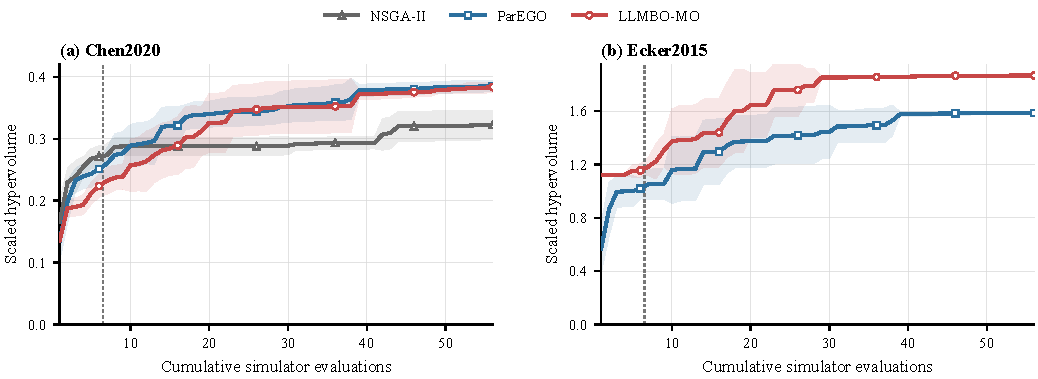
\includegraphics[width=0.96\textwidth]{Section/figures/benchmark_hv.pdf}
\caption{Fixed-budget search progress over seeds 8409--8413. Lines are
five-seed means and bands are $\pm1$ sample standard deviation; the vertical
dashed line marks the end of the six-point initialization. (a) Chen2020,
including NSGA-II truncated to 56 evaluations. (b) Ecker2015. Each panel uses
its own fixed ideal/reference box from~\eqref{eq:scaled_hv}; absolute sHV
values should not be compared across panels.}
\label{fig:benchmark_hv}
\end{figure*}

\subsection{Pareto Sets and Charging Trajectories}

To inspect the solutions rather than only their volume, Fig.~\ref{fig:pareto}
shows the nondominated sets from a separate Chen2020 seed-8409 archive. This
illustrative run is not used to compute Table~\ref{tab:benchmark_results}.
The three projections show the same full three-objective Pareto sets; a point
that appears dominated in one projection can remain nondominated because of
the omitted objective.

\begin{figure*}[!t]
\centering
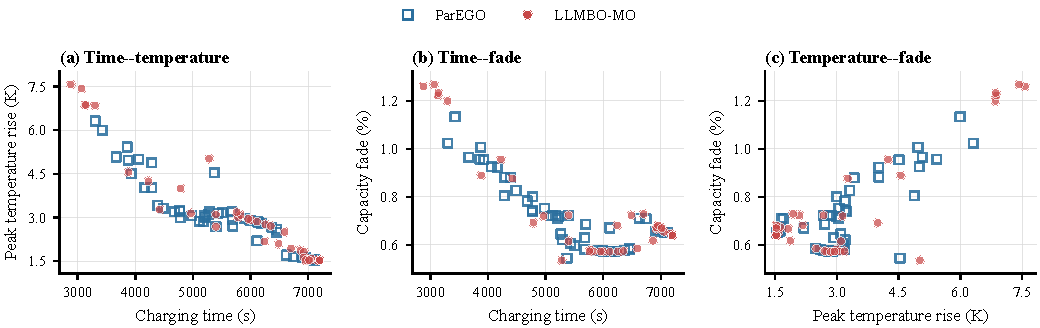
\includegraphics[width=0.95\textwidth]{Section/figures/pareto_projections.pdf}
\caption{Pairwise projections of the Chen2020 seed-8409 nondominated sets
after 56 evaluations. ParEGO returns 45 points and LLMBO-MO returns 37 points.
All markers are nondominated in the full three-objective space.}
\label{fig:pareto}
\end{figure*}

Table~\ref{tab:protocols} selects three archived LLMBO-MO points spanning the
time--temperature trade-off. They are replayed with the same simulator in
Fig.~\ref{fig:charging_profiles}. The voltage traces remain below the 4.4-V
limit. The high-current protocol reaches the target state of charge sooner
but produces the largest temperature rise; the lower-current protocols
reduce thermal stress at the cost of longer charging time.

\begin{table}[!t]
\caption{Illustrative Chen2020 LLMBO-MO Protocols, Seed 8409}
\label{tab:protocols}
\centering
\scriptsize
\setlength{\tabcolsep}{1.6pt}
\begin{tabular}{@{}lccccc@{}}
\toprule
Protocol & $(I_1,I_2,I_3)$ (A) & $(\Delta s_1,\Delta s_2)$
& $t_c$ (s) & $\Delta T_p$ (K) & $Q_s$ (\%) \\
\midrule
Fast & $(6,5,3)$ & $(0.400,0.300)$ & 2880 & 7.567 & 1.261 \\
Intermediate & $(2,2,3)$ & $(0.320,0.118)$ & 6112 & 2.857 & 0.571 \\
Low-temperature & $(2,2,2)$ & $(0.100,0.300)$ & 7200 & 1.529 & 0.640 \\
\bottomrule
\end{tabular}
\end{table}

\begin{figure*}[!t]
\centering
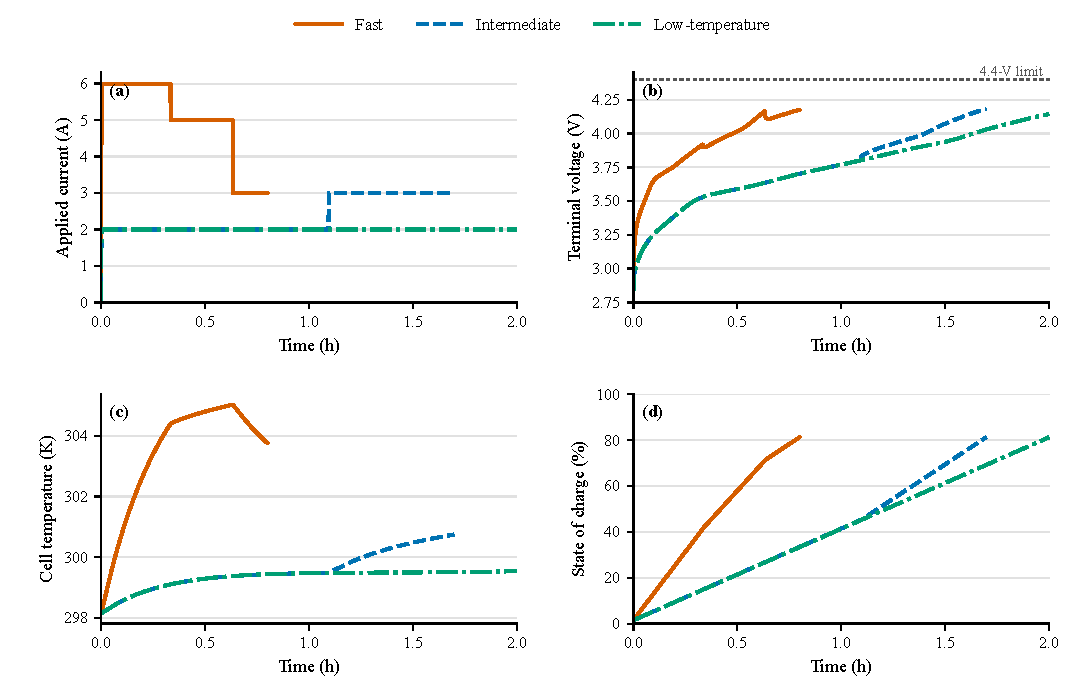
\includegraphics[width=0.93\textwidth]{Section/figures/charging_profiles.pdf}
\caption{Simulator replay of the three LLMBO-MO protocols in
Table~\ref{tab:protocols}: (a) applied current, (b) terminal voltage,
(c) cell temperature, and (d) state of charge. These are simulated
trajectories, not physical-cell measurements.}
\label{fig:charging_profiles}
\end{figure*}

\subsection{Ablation Study}

% Source: adaptive4_5seeds_50iter_deepseek_v3_2026_05_22
The ablation uses only the matched May 22, 2026 Chen2020
\texttt{adaptive4} archive. All four variants share the same seeds,
56-evaluation budget, simulator, and reporting code. This excludes the
four-group summary elsewhere in the archive because that summary combines
runs from different batches.

\begin{table}[!t]
\caption{Same-Batch Chen2020 Ablation over Five Seeds}
\label{tab:ablation}
\centering
\footnotesize
\setlength{\tabcolsep}{3.0pt}
\begin{tabular}{@{}lccc@{}}
\toprule
Variant & Final sHV & $\Delta$ vs. baseline & Wins \\
\midrule
Baseline & \AblationBaselineMean\,$\pm$\,\AblationBaselineStd & -- & -- \\
Warm start & \textbf{\AblationWarmMean}\,$\pm$\,\AblationWarmStd
& +\AblationWarmDelta & 4/5 \\
Region guidance & \AblationRegionMean\,$\pm$\,\AblationRegionStd
& +\AblationRegionDelta & 4/5 \\
Full LLMBO & \AblationFullMean\,$\pm$\,\textbf{\AblationFullStd}
& +\AblationFullDelta & 3/5 \\
\bottomrule
\end{tabular}
\end{table}

Warm starting gives the largest mean sHV in this batch. The full method is
lower by only 0.0002 and has the smallest sample standard deviation. Region
guidance alone improves the mean by 0.0026 but also has the largest
variation. These data support warm starting as the more repeatable source of
gain; they do not establish that iteration-level guidance improves every
seed.

\begin{figure*}[!t]
\centering
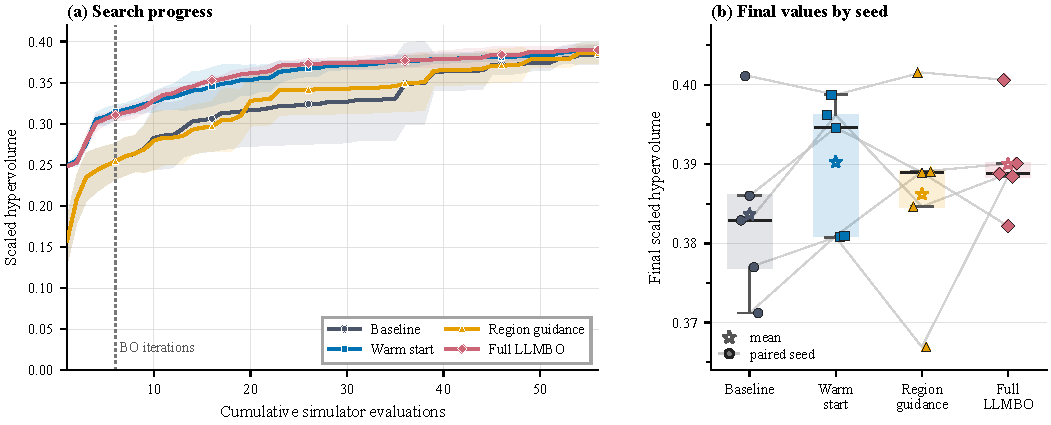
\includegraphics[width=0.96\textwidth]{Section/figures/ablation_same_batch.pdf}
\caption{Same-batch Chen2020 ablation over seeds 8409--8413.
(a) Five-seed mean search trajectories with $\pm1$ sample-standard-deviation
bands. (b) Final values; markers are individual seeds, gray lines preserve
the pairing, and stars denote means.}
\label{fig:ablation}
\end{figure*}

\subsection{Runtime and Scope}

The archived Chen2020 timing report records
$252.4\pm17.7$~s for ParEGO and $440.3\pm31.3$~s for LLMBO-MO at 56
evaluations. The latter is 1.74 times slower because wall time includes LLM
requests and region-processing logic. NSGA-II requires
$194.3\pm11.8$~s for its complete 60-evaluation run. Hardware metadata was
not stored with the report, so these values document overhead within the
archive rather than provide a portable runtime benchmark.

The present evidence is limited to simulator evaluations, five seeds, and
two parameterizations. In particular, Fig.~\ref{fig:charging_profiles}
checks feasibility under the model but does not replace experimental
validation against measured voltage and temperature trajectories.

\clearpage
